\chapter{HASIL YANG DIHARAPKAN}

\section{Hasil yang Diharapkan dari Penelitian}

Hasil yang diharapkan dari penelitian ini adalah terciptanya sebuah sistem robotik berbasis
\emph{Human-Robot Interaction} (HRI) yang memungkinkan operator (manusia) untuk berperan aktif
dalam proses pemilihan objek yang akan diambil oleh robot lengan yang terpasang pada robot
\emph{quadruped}. Dengan adanya \emph{Graphical User Interface} (GUI), sistem ini akan menampilkan
deteksi objek dalam bentuk bounding box, sehingga operator dapat memilih objek secara langsung melalui
antarmuka yang intuitif, menghilangkan kemungkinan kesalahan robot dalam pengambilan keputusan atau
memilih objek yang tidak diinginkan. Setelah pemilihan objek dilakukan, sistem akan mengoptimalkan
\emph{pose grasping} menggunakan GraspNet untuk memastikan genggaman yang stabil dan akurat. Penelitian
ini juga menargetkan pengembangan algoritma sistem \emph{task-level} yang mampu mengintegrasikan berbagai komponen,
termasuk persepsi visual, pemrosesan data \emph{grasping}, kendali robot lengan, serta navigasi \emph{quadruped},
sehingga robot dapat bekerja secara efisien dalam menjalankan tugasnya.

\section{Hasil Pendahuluan}
Sejauh ini, penulis telah melakukan studi literatur terkait \emph{tools} dan \emph{library} yang digunakan dalam penelitian ini.
\emph{Tools} dan \emph{library} tersebut antara lain GraspNet sebagai \emph{framework} berbasis \emph{deep learning} yang dirancang untuk
melakukan prediksi \emph{pose grasping} bagi lengan robot, ROS sebagai sebuah \emph{framework open-source} yang membantu pengembangan,
pengendalian, serta komunikasi antar komponen sistem robotik, serta QT sebagai \emph{framework} pengembangan aplikasi yang digunakan
untuk membangun antarmuka grafis (GUI). Selain itu, studi literatur juga dilakukan terkait \emph{hardware} yang akan digunakan dalam penelitian,
yaitu kamera Intel Realsense, robot \emph{quadruped} DeepRobotics Lite3, serta robot lengan (Open Manipulator - X).

Selanjutnya, penulis telah mengerjakan desain mounting kamera realsense yang dipasang di ujung robot lengan.
Pengerjaan desain dilakukan dengan onshape, lalu dicetak dengan 3d printer. Desain dibuat dengan memperhatikan
beberapa faktor seperti kemudahan instalasi dan kejelasan pandangan kamera. Selain itu, dengan kamera yang
berada di ujung, robot dapat mengendalikan arah kamera sesuai dengan arah gripper. Berikut merupakan hasil desain mounting
dan hasil cetaknya.

aaaaaaaaaaaaaaaaaa GAMBAR aaaaaaaaaaaaaaaaaa

Dalam proses implementasi GraspNet, penulis berada dalam tahap konfigurasi kamera yang akan digunakan yaitu Intel Realsense.
Kamera ini merupakan hal dasar yang diperlukan untuk melakukan \emph{grasp detection}. Terdapat tiga output yang dikeluarkan oleh kamera,
yaitu \emph{RGB Stream}, \emph{Depth Stream}, dan Odometri. Dari ketiganya, hanya dua yang digunakan nantinya yaitu \emph{rgb stream}
dan \emph{depth stream}.
\begin{figure}[h]
    \centering
    \begin{minipage}{0.48\columnwidth}
        \centering
        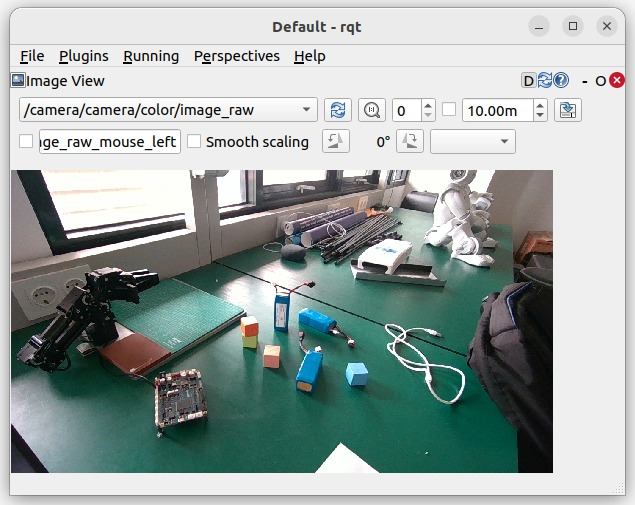
\includegraphics[width=\linewidth]{gambar/rgb stream.jpeg}
        \caption{stream rgb}
        \label{fig:rgb_stream}
    \end{minipage}
    \hfill
    \begin{minipage}{0.48\columnwidth}
        \centering
        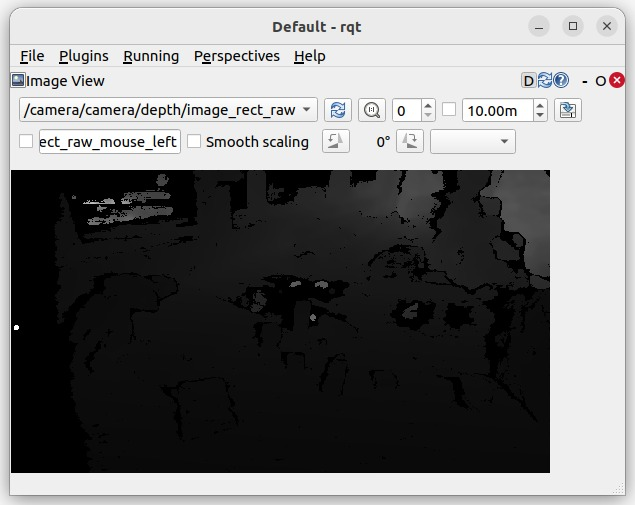
\includegraphics[width=\linewidth]{gambar/depth stream.jpeg}
        \caption{stream depth}
        \label{fig:depth_stream}
    \end{minipage}
\end{figure}
\begin{figure} [H] \centering
    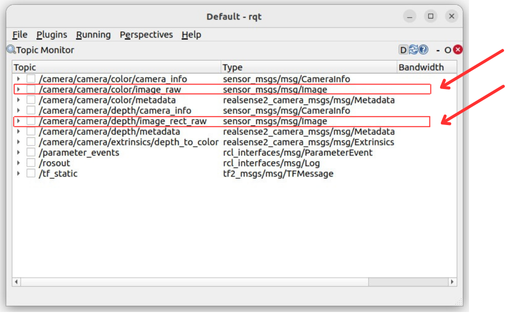
\includegraphics[scale=0.6]{gambar/topic realsense anotated.png}
    \caption{Topic terkait Realsense}
    \label{fig:realsense_topic}
\end{figure}
Penulis telah melakukan instalasi ROS-wrapper berbentuk package realsense2\_camera untuk kedua \emph{stream} ini.
Dari gambar \ref{fig:realsense_topic} dapat dilihat terdapat dua topic ROS yang merepresentasikan \emph{stream} untuk rgb dan depth. Dengan kedua topic ini,
maka data streamnya dapat diteruskan ke program GraspNet sebagai data persepsi untuk dilakukan \emph{grasp detection}. Sedangkan gambar \ref{fig:rgb_stream}
dan \ref{fig:depth_stream} memperlihatkan hasil streaming dari kamera realsense yang ditampilkan dengan rqt tools.
Berikut merupakan diagram input-output yang merepresentasikan cara kerja GraspNet.

aaaaaaaaaaaaaaaaaa GAMBAR aaaaaaaaaaaaaaaaaa

Selain itu, penulis juga telah mengintegrasikan sistem \emph{motion planning} untuk robot lengan. Sistem \emph{motion planning} yang digunakan adalah MoveIt,
sedangkan robot yang digunakan untuk percobaan ini adalah Open Manipulator - X. Sistem \emph{motion planning} ini merupakan sistem yang membuat
peneliti dapat mengatur bagaimana robot lengan bergerak. Karena menggunakan ROS, robot lengan digerakkan dengan cara mengirimkan informasi
ke beberapa topic, service, dan action yang terkait seperti di bawah ini.
\begin{figure} [H] \centering
    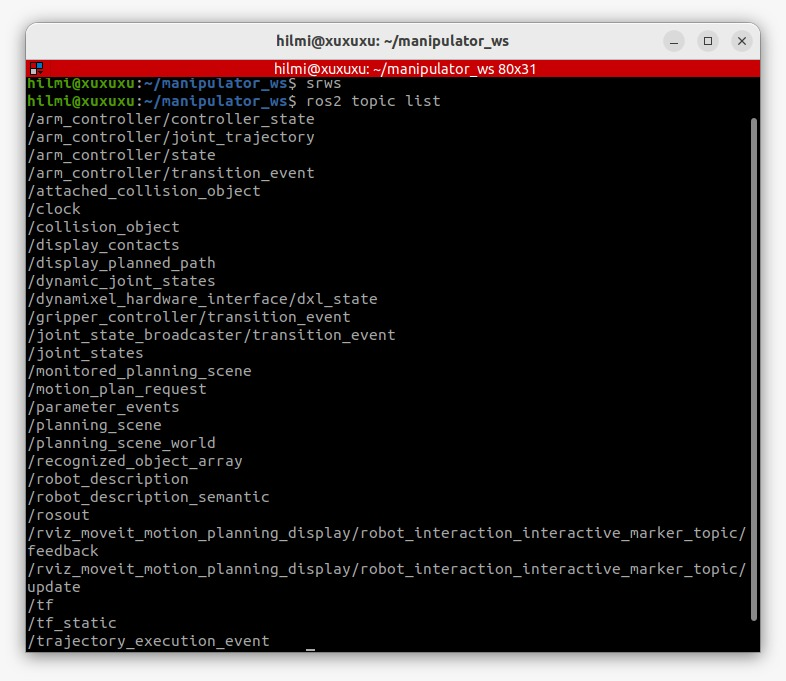
\includegraphics[scale=0.3]{gambar/moveit topic.jpeg}
    \caption{Topic MoveIt}
    \label{fig:moveit_topic}
  \end{figure}
\begin{figure} [H] \centering
    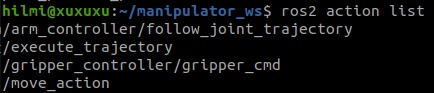
\includegraphics[scale=0.4]{gambar/moveit actions.jpeg}
    \caption{Actions MoveIt}
    \label{fig:moveit_actions}
\end{figure}
Selain itu, OpenCR sebagai perantara laptop yang menjalankan ROS dengan robot lengan harus diflash \emph{firmware} yang berfungsi sebagai
USB to DXL. Dalam sistem ROS, komunikasi dengan motor Dynamixel dilakukan melalui protokol serial,
sedangkan sebagian besar komputer hanya memiliki antarmuka USB. USB to DXL berfungsi sebagai jembatan dengan mengonversi data dari
USB ke protokol komunikasi yang digunakan oleh motor Dynamixel. Pada Open Manipulator yang dikendalikan dengan ROS,
USB to DXL memungkinkan komunikasi antara PC atau SBC dengan motor Dynamixel melalui port USB, menggunakan perangkat lunak
seperti dynamixel\_workbench atau ros\_control untuk mengirim perintah gerakan,
membaca status motor, dan menjalankan algoritma kontrol dalam lingkungan ROS.
\begin{figure} [H] \centering
    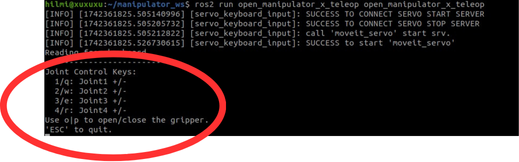
\includegraphics[scale=0.8]{gambar/keyboard control anotated.png}
    \caption{Kontrol dengan keyboard}
    \label{fig:keyboard_control}
  \end{figure}
\begin{figure} [H] \centering
    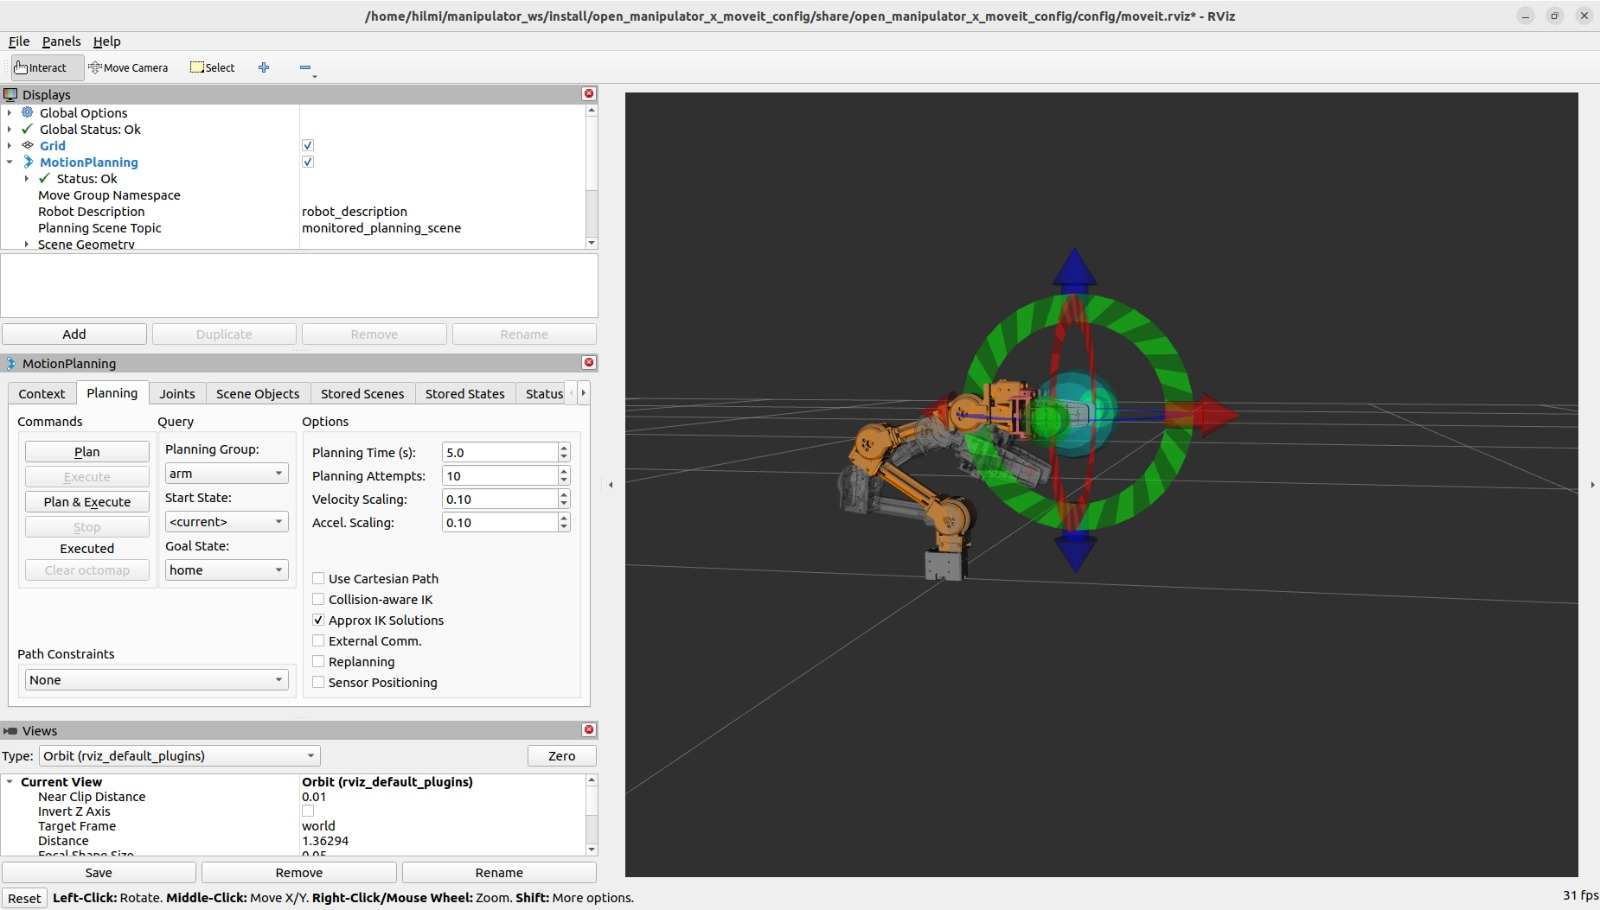
\includegraphics[scale=0.3]{gambar/moveit gui.jpeg}
    \caption{Kontrol dengan GUI}
    \label{fig:moveit_gui}
\end{figure}
Dalam pengujian sistem \emph{motion control}, robot lengan dikontrol dengan dua cara yaitu menggunakan keyboard dan GUI MoveIt.
Dalam kontrol keyboard, robot dikendalikan dengan mengontrol secara terpisah tiap motor yang ada.
Seperti yang terlihat pada gambar \ref{fig:keyboard_control}, terdapat 4 motor yang berperan sebagai joint
dan 1 motor yang berperan sebagai gripper. Kelima motor tersebut dikontrol secara langsung oleh tombol-tombol keyboard.
Dalam kontrol GUI di gambar \ref{fig:moveit_gui}, robot dapat melakukan \emph{motion planning} sesuai dengan yang direncanakan.
Peneliti dapat merencanakan pergerakan dengan cara menggerakkan tampilan robot lengan yang ada di GUI. Selanjutnya,
tombol plan \& execute dapat ditekan agar robot di dunia nyata mengikuti pergerakan yang telah direncanakan tersebut.

\emph{Motion planning} ini merupakan salah satu tahap yang wajib dalam melakukan grasping.
Hal ini karena GraspNet sendiri belum include dengan \emph{motion planning}. Output dari GraspNet
adalah mendapat informasi 6-dof untuk melakukan grasping, sedangkan untuk robot lengan menuju posisi
target 6-dof tersebut menggunakan sistem di luar GraspNet. Dalam hal ini, yaitu menggunakan sistem \emph{motion
planning} MoveIt.

[atas udah, tinggal ini ke bawah] op3 kekecilan jadi pake robot arm yg sekarang
penyesuaiaan base mounting
program pemilihan objek